\documentclass{beamer}
\usepackage{amsmath}
\usepackage{amssymb}
\usepackage{graphicx}
\usepackage{tikz}
\usepackage{multicol}
\usetheme{Madrid}
\usecolortheme{default}

\title{GED Math: Ratios, Proportions, and Percents}

\date{\today}

\begin{document}

\frame{\titlepage}

%-------------------------------------------
% Lesson 1: Ratios
%-------------------------------------------
\begin{frame}{Lesson 1: Understanding Ratios}
\textbf{Objective:} Understand how to express and simplify ratios.
\begin{itemize}
    \item A \textbf{ratio} compares two quantities by division.
    \item Ratios can be written as $a:b$, $a/b$, or "a to b".
    \item Simplify a ratio the same way you simplify a fraction.
\end{itemize}
\vspace{1em}
\begin{center}
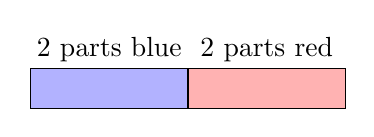
\begin{tikzpicture}
    % Ratio bar model example
    \draw[fill=blue!30] (0,0) rectangle (2,0.5);
    \draw[fill=red!30] (2,0) rectangle (4,0.5);
    \node at (1,0.75) {2 parts blue};
    \node at (3,0.75) {2 parts red};
\end{tikzpicture}
\end{center}
\end{frame}

\begin{frame}{Worked Examples: Ratios}
\textbf{Example 1:} Simplify $12:16$.\\
\textit{Solution:} $\frac{12}{16} = \frac{3}{4}$, so the ratio is $3:4$.

\vspace{0.5em}
\textbf{Example 2:} Express 8 red marbles to 12 blue marbles as a ratio.\\
\textit{Solution:} $8:12 = 2:3$.

\vspace{0.5em}
\textbf{Example 3:} Write the ratio of 50 cm to 2 m.\\
\textit{Solution:} Convert 2 m = 200 cm. Ratio = $50:200 = 1:4$.

\vspace{0.5em}
\textbf{Example 4:} If a class has 10 boys and 15 girls, ratio of boys to total?\\
$10:(10+15)=10:25=2:5$.

\vspace{0.5em}
\textbf{Example 5:} A recipe calls for 4 cups of flour and 2 cups of sugar. Simplify.\\
$4:2=2:1$.
\end{frame}

%-------------------------------------------
% Lesson 2: Proportions
%-------------------------------------------
\begin{frame}{Lesson 2: Understanding Proportions}
\textbf{Objective:} Solve problems involving proportions.
\begin{itemize}
    \item A \textbf{proportion} states that two ratios are equal: $\frac{a}{b} = \frac{c}{d}$.
    \item Use \textbf{cross multiplication}: $a \times d = b \times c$.
\end{itemize}
\vspace{1em}
\begin{center}
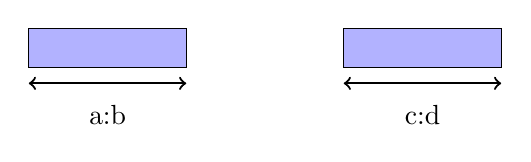
\begin{tikzpicture}
    % proportion bar model
    \draw[fill=blue!30] (0,0) rectangle (2,0.5);
    \draw[fill=blue!30] (4,0) rectangle (6,0.5);
    \draw[<->,thick] (0,-0.2)--(2,-0.2);
    \draw[<->,thick] (4,-0.2)--(6,-0.2);
    \node at (1,-0.6) {a:b};
    \node at (5,-0.6) {c:d};
\end{tikzpicture}
\end{center}
\end{frame}

\begin{frame}{Worked Examples: Proportions}
\textbf{Example 1:} $\frac{3}{4} = \frac{x}{12}$\\
$3 \times 12 = 4x \Rightarrow 36 = 4x \Rightarrow x = 9$

\vspace{0.5em}
\textbf{Example 2:} $\frac{8}{x} = \frac{2}{3}$\\
$8 \times 3 = 2x \Rightarrow 24 = 2x \Rightarrow x = 12$

\vspace{0.5em}
\textbf{Example 3:} If 5 pencils cost \$2.50, how much do 8 pencils cost?\\
$\frac{5}{2.50} = \frac{8}{x} \Rightarrow 5x = 20 \Rightarrow x = 4.00$

\vspace{0.5em}
\textbf{Example 4:} $\frac{7}{14} = \frac{x}{28}$\\
$7 \times 28 = 14x \Rightarrow 196 = 14x \Rightarrow x = 14$

\vspace{0.5em}
\textbf{Example 5:} If 3 gallons of paint cover 900 sq ft, how many sq ft for 5 gallons?\\
$\frac{3}{900} = \frac{5}{x} \Rightarrow 3x = 4500 \Rightarrow x = 1500$ sq ft.
\end{frame}

%-------------------------------------------
% Lesson 3: Percents
%-------------------------------------------
\begin{frame}{Lesson 3: Understanding Percents}
\textbf{Objective:} Solve problems involving percent, part, and whole.
\begin{itemize}
    \item Percent means \textbf{per hundred}. $50\% = \frac{50}{100} = 0.5$.
    \item Use the formula: \textbf{Part = Percent $\times$ Whole}.
\end{itemize}
\vspace{1em}
\begin{center}
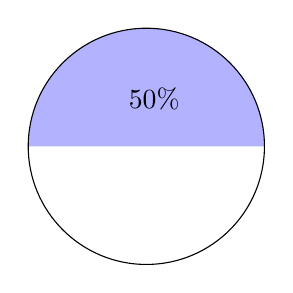
\begin{tikzpicture}
    % Percent circle diagram
    \fill[blue!30] (0,0) -- (0:1.5cm) arc (0:180:1.5cm) -- cycle;
    \draw (0,0) circle (1.5cm);
    \node at (0.1,0.6) {50\%};
\end{tikzpicture}
\end{center}
\end{frame}

\begin{frame}{Worked Examples: Percents}
\textbf{Example 1:} What is 25\% of 200?\\
$= 0.25 \times 200 = 50$.

\vspace{0.5em}
\textbf{Example 2:} 40 is what percent of 80?\\
$\frac{40}{80} = 0.5 = 50\%$.

\vspace{0.5em}
\textbf{Example 3:} 20 is 25\% of what number?\\
$20 = 0.25x \Rightarrow x = 80$.

\vspace{0.5em}
\textbf{Example 4:} A $60$ item is discounted by $15\%$. Find sale price.\\
$0.15 \times 60 = 9$. New price = $60 - 9 = 51$.

\vspace{0.5em}
\textbf{Example 5:} A $1200$ computer has 13\% tax. Total cost?\\
$0.13 \times 1200 = 156$. Total = $1356$.
\end{frame}

%-------------------------------------------
% Lesson 4: Applications & Mixed Problems
%-------------------------------------------
\begin{frame}{Lesson 4: Applications of Ratios, Proportions, and Percents}
\textbf{Objective:} Apply ratios, proportions, and percents in real-world problems.
\begin{itemize}
    \item Combine skills: compare quantities, solve for unknowns, and interpret percent changes.
\end{itemize}
\vspace{1em}
\begin{center}
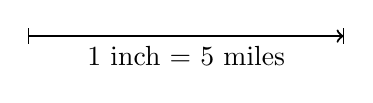
\begin{tikzpicture}
    % Real world problem illustration: map scale
    \draw[thick,->] (0,0) -- (4,0) node[midway,below]{1 inch = 5 miles};
    \draw (0,-0.1)--(0,0.1);
    \draw (4,-0.1)--(4,0.1);
\end{tikzpicture}
\end{center}
\end{frame}

\begin{frame}{Worked Examples: Applications}
\textbf{Example 1:} A map scale shows $1$ inch = $5$ miles. How many miles is $3.5$ inches?\\
$\frac{1}{5} = \frac{3.5}{x} \Rightarrow x = 17.5$ miles.

\vspace{0.5em}
\textbf{Example 2:} A population grows from 800 to 1000. Find percent increase.\\
$\frac{200}{800} = 0.25 = 25\%$.

\vspace{0.5em}
\textbf{Example 3:} A student answered 42 of 50 questions correctly.\\
$\frac{42}{50} = 0.84 = 84\%$.

\vspace{0.5em}
\textbf{Example 4:} A recipe for 6 servings uses 3 cups of rice. How much for 10 servings?\\
$\frac{6}{3} = \frac{10}{x} \Rightarrow x = 5$ cups.

\vspace{0.5em}
\textbf{Example 5:} A car travels 240 miles on 8 gallons. How far on 10 gallons?\\
$\frac{8}{240} = \frac{10}{x} \Rightarrow 8x = 2400 \Rightarrow x = 300$ miles.
\end{frame}

\begin{frame}{Review Summary}
\begin{itemize}
    \item Ratios compare quantities visually and numerically.
    \item Proportions show equivalent relationships.
    \item Percents express parts per hundred with circle or bar visuals.
    \item Apply all three concepts in real-world problems.
\end{itemize}
\end{frame}

\end{document}
